‫\فصل{سند موارد کاربرد}
‫\قسمت{توصیف کنش‌گر‌ها}
‫
‫\شروع{لوح}[ht]
‫\تنظیم‌ازوسط
‫
‫\شروع{جدول}{|p{3cm}|p{9cm}|}
‫\خط‌پر 
‫\سیاه کنشگر & \سیاه توصیف \\ 
‫\خط‌پر
‫صاحب کانال & کسی است که کانال جدید در سامانه می‌سازد و می‌تواند محتوا بارگذاری کند و از میان اعضای کانال شخص یا اشخاصی را به عنوان مدیر انتخاب نماید. تمامی حقوق مادی حاصله از کسب درآمد برای این فرد است و این فرد درآمد به دست آمده را در بین مدیران کانال تقسیم می‌کند.\\ 
‫
‫\خط‌پر
‫\پایان{جدول}
‫‫\شرح{توصیف کنشگر صاحب کانال}
‫\برچسب{جدول:توصیف کنشگر صاحب کانال}
‫\پایان{لوح}
‫\FloatBarrier
‫\شروع{لوح}[ht]
‫\تنظیم‌ازوسط
‫
‫\شروع{جدول}{|p{3cm}|p{9cm}|}
‫\خط‌پر 
‫\سیاه کنشگر & \سیاه توصیف \\ 
‫\خط‌پر
‫مدیر کانال & کسی است که محتوای تولید شده را بارگذاری می‌کند و بر کانال نظارت می‌کند و درصدی از درآمد کانال برای اوست و توسط صاحب کانال انتخاب می‌شود\\ 
‫
‫\خط‌پر
‫\پایان{جدول}
‫‫\شرح{توصیف کنشگر مدیر کانال}
‫
‫\برچسب{جدول:توصیف کنشگر مدیر کانال}
‫\پایان{لوح}
‫‫\FloatBarrier
‫
‫\شروع{لوح}[ht]
‫\تنظیم‌ازوسط
‫\شروع{جدول}{|p{3cm}|p{9cm}|}
‫\خط‌پر 
‫\سیاه کنشگر & \سیاه توصیف \\ 
‫\خط‌پر
‫عضو ویژه کانال & کسی است که عضو کانال است و از محتوای بارگذاری شده استفاده می‌کند. این عضو عضو ویژه است بدین معنی که می‌تواند از محتوای پریمیوم کانال استفاده نماید. هر عضوی از کانال که اشتراک پولی بخرد می‌تواند از محتوای غیر رایگان استفاده کند. علاوه بر محتوای پولی امکان استفاده از محتوای عادی را نیز دارد.\\ 
‫
‫\خط‌پر
‫\پایان{جدول}
‫‫\شرح{توصیف کنشگر عضو ویژه کانال}
‫
‫\برچسب{جدول:توصیف کنشگر عضو ویژه کانال}
‫\پایان{لوح}
‫‫\
‫
‫\شروع{لوح}[ht]
‫\تنظیم‌ازوسط
‫\شروع{جدول}{|p{3cm}|p{9cm}|}
‫\خط‌پر 
‫\سیاه کنشگر & \سیاه توصیف \\ 
‫\خط‌پر
‫عضو عادی کانال & کسی است که عضو کانال است و از محتوای بارگذاری شده استفاده می‌کند. این عضو فقط اجازه استفاده از محتوای عادی و رایگان کانال را دارد و نمی‌تواند از محتوای پولی بارگذاری شده استفاده نماید. صرفا میتواند یک خلاصه و عنوان از محتوای پولی ببیند.\\ 
‫
‫\خط‌پر
‫\پایان{جدول}
‫‫\شرح{توصیف کنشگر عضو عادی کانال}
‫
‫\برچسب{جدول:توصیف کنشگر عضو عادی کانال}
‫\پایان{لوح}
‫‫\FloatBarrier
‫
‫\شروع{لوح}[ht]
‫\تنظیم‌ازوسط
‫\شروع{جدول}{|p{3cm}|p{9cm}|}
‫\خط‌پر 
‫\سیاه کنشگر & \سیاه توصیف \\ 
‫\خط‌پر
‫صاحبان محصول قاصدک & کسانی که در توسعه نرم افزار قاصدک نقش داشته‌اند و آن را به وجود آورده‌اند منظور شرکت ایجاد نرم افزار می‌باشد.\\ 
‫
‫\خط‌پر
‫\پایان{جدول}
‫‫\شرح{توصیف کنشگر صاحبان محصول قاصدک}
‫
‫\برچسب{جدول:توصیف کنشگر صاحبان محصول قاصدک}
‫\پایان{لوح}
‫\FloatBarrier
‫
‫
‫\شروع{لوح}[ht]
‫\تنظیم‌ازوسط
‫\شروع{جدول}{|p{3cm}|p{9cm}|}
‫\خط‌پر 
‫\سیاه کنشگر & \سیاه توصیف \\ 
‫\خط‌پر
‫سیستم بانکی & شامل بانک، حساب‌های بانکی و سیستم درگاه پرداخت آنلاین است که برای پرداخت آنلاین و انجام کار‌های مالی به آن مراجعه کرد.\\ 
‫
‫\خط‌پر
‫\پایان{جدول}
‫‫\شرح{توصیف کنشگر سسیستم بانکی}
‫
‫\برچسب{جدول:توصیف کنشگر سسیستم بانکی}
‫\پایان{لوح}
‫‫\FloatBarrier
‫
‫\زیرقسمت{نمودار موارد کاربرد}
‫سیستم ما از پنج زیر سیستم مدیریت کاربران، مدیریت کانال، مدیریت محتوا، پرداخت و مالی و پیشنهاد تشکیل شده است که در هر کدام از این زیردامنه‌ها مواردکاربرد مربوط به آن‌ها قرار گرفته است، نمودار این موارد کاربرد به صورت زیر است:
‫\\
‫
‫\شروع{شکل}[ht]
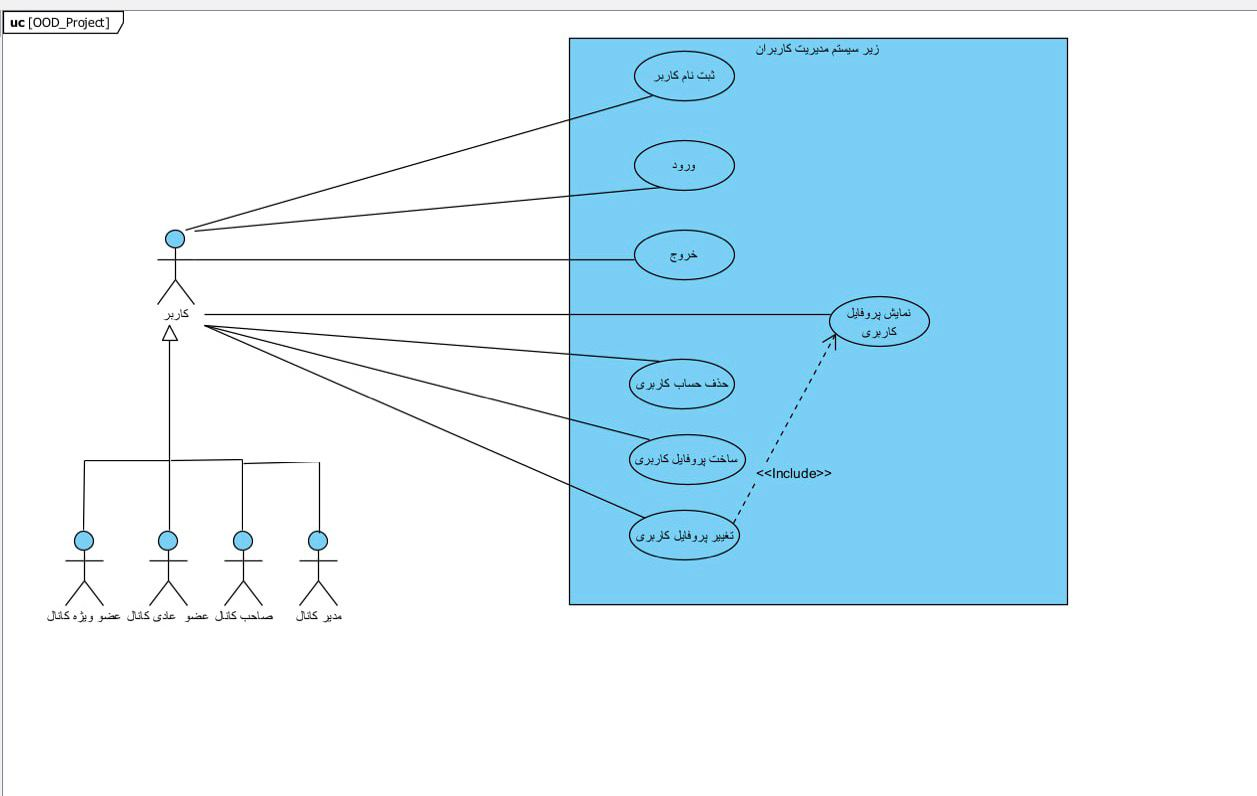
\includegraphics[scale=0.3]{figs/user_subsys.jpeg}
‫\شرح{نمودار کاربرد زیرسیستم مدیریت کاربران}
‫\برچسب{شکل:نمودار کاربرد زیرسیستم مدیریت کاربران}
‫\پایان{شکل}
\FloatBarrier
‫\شروع{شکل}[ht]
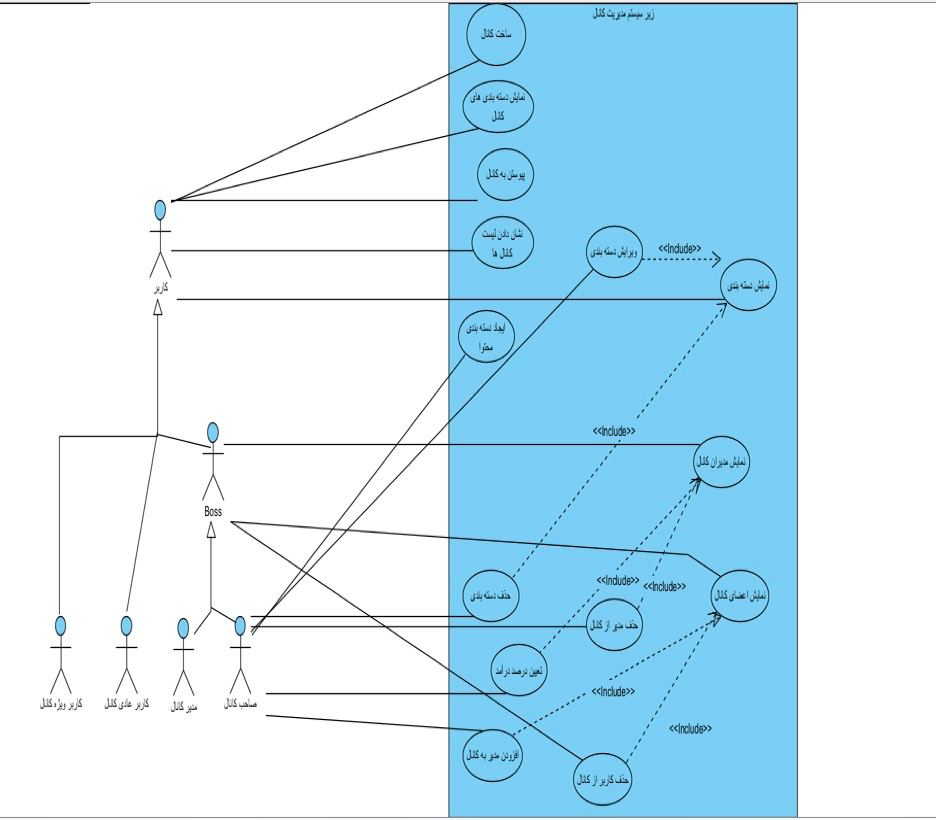
\includegraphics[scale=0.4]{figs/channel_subsys.jpeg}
‫\شرح{نمودار کاربرد زیرسیستم مدیریت کانال}
‫\برچسب{شکل:نمودار کاربرد زیرسیستم مدیریت کانال}
‫\پایان{شکل}
‫‫\FloatBarrier
‫
‫\شروع{شکل}[ht]
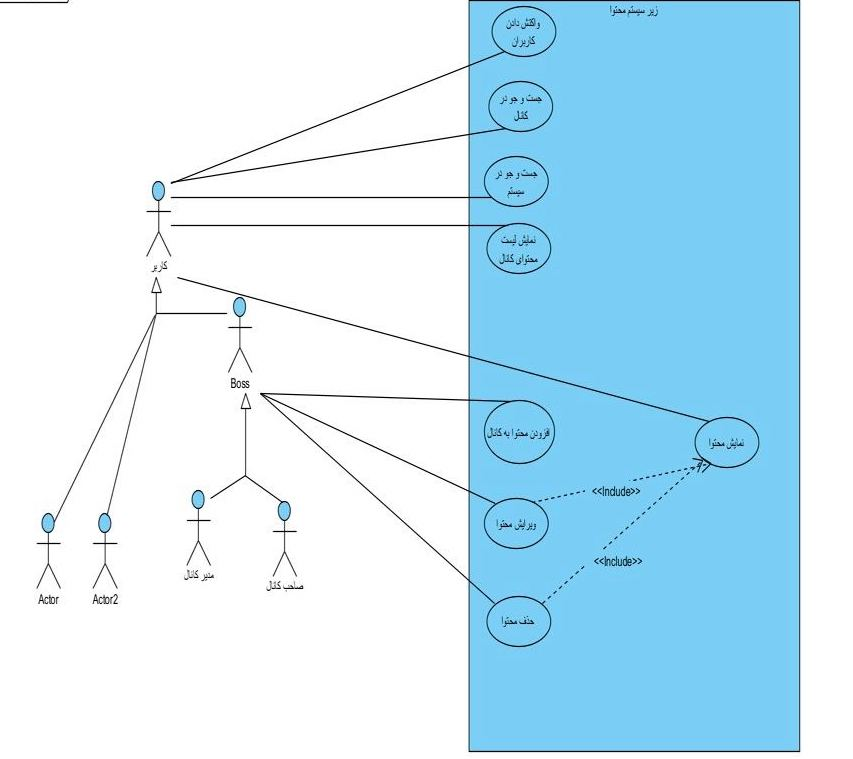
\includegraphics[scale=0.4]{figs/content_subsys.jpeg}
‫\شرح{نمودار کاربرد زیرسیستم محتوا}
‫\برچسب{شکل:نمودار کاربرد زیرسیستم محتوا}
‫\پایان{شکل}
‫
‫\FloatBarrier
‫
‫\شروع{شکل}[ht]
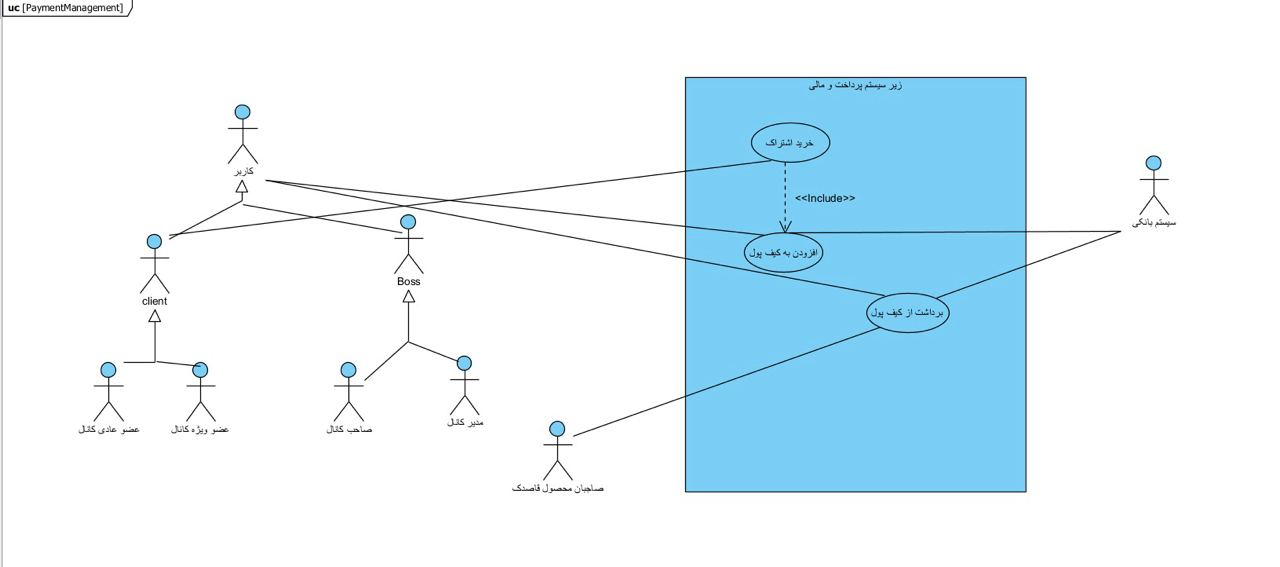
\includegraphics[scale=0.4]{figs/finance_subsys.jpeg}
‫\شرح{نمودار کاربرد زیرسیستم پرداخت و مالی}
‫\برچسب{شکل:نمودار کاربرد زیرسیستم پرداخت و مالی}
‫\پایان{شکل}
‫\
‫\
‫\
‫‫\FloatBarrier
‫


‫\شروع{شکل}[ht]
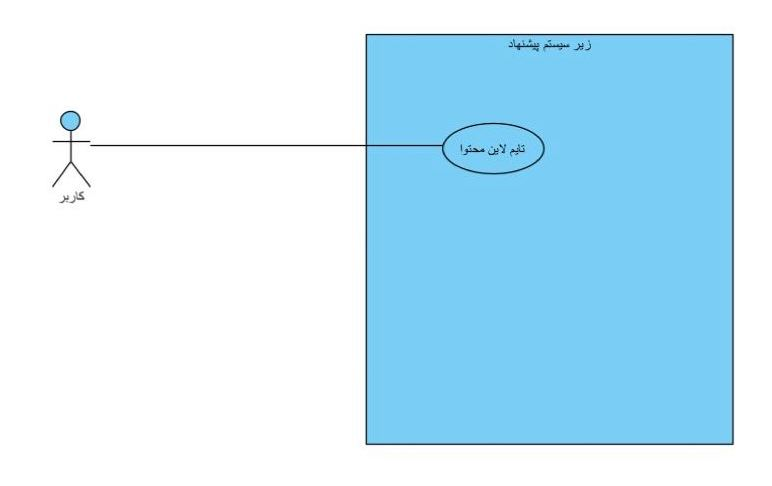
\includegraphics[scale=0.4]{figs/suggest_subsys.jpeg}
‫\شرح{نمودار کاربرد زیرسیستم پیشنهاد}
‫\برچسب{شکل:نمودار کاربرد زیرسیستم پیشنهاد}
‫\پایان{شکل}
‫‫\FloatBarrier
‫
‫\زیرقسمت{توصیف موارد کاربرد}
‫حال به توصیف دقیق هر کدام از موارد کاربرد به ترتیب می‌پردازیم.
‫
‫\زیرقسمت{زیرسیستم کاربر}
‫
‫
‫\شروع{لوح}[ht]
‫\تنظیم‌ازوسط
‫
‫\شروع{جدول}{|p{3cm}|p{9cm}|}
‫\خط‌پر 
‫ مورد کاربرد &  ثبت‌نام \\ 
‫\خط‌پر
‫شناسه & ۱\\ 
‫\خط‌پر
‫خلاصه & کاربر با ورود اطلاعات کاربری(ایمیل یا شماره تلفن) به همراه رمز عبور یک حساب کاربری جدید می‌سازد.\\
‫\خط‌پر
‫عامل اصلی & کاربر\\
‫\خط‌پر
‫عامل فرعی & ندارد\\
‫\خط‌پر
‫شرایط اولیه & ندارد\\
‫\خط‌پر
‫روند اصلی & 
‫\شروع{شمارش}
‫\فقره این مورد کاربرد با درخواست کاربر برای ثبت حساب کاربری در سیستم آغاز می‌گردد.
‫\فقره از کاربر مورد نظر اطلاعات کاربری(ایمیل یا شماره تلفن) و رمز عبور دریافت می‌گردد.
‫\فقره سامانه اطلاعات کاربری را اعتبار سنجی می‌کند.
‫\فقره سامانه بررسی می‌کند که کاربری با چنین شماره تلفن و ایمیلی در سامانه موجود است یا خیر.
‫\فقره حساب کاربری برای کاربر ساخته می‌شود.
‫\پایان{شمارش}
‫\\
‫\خط‌پر
‫
‫‫شرایط نهایی & حساب کاربری برای فرد ایجاد می‌شود\\
‫\خط‌پر
‫روند‌های جایگزین & ثبت نام: ورود اطلاعات نامعتبر، ثبت نام: وجود حساب کاربری با مشخصات مشابه
‫\\
‫‫\خط‌پر
‫
‫\پایان{جدول}
‫‫\شرح{توصیف مورد کاربرد ثبت‌نام}
‫\برچسب{جدول:توصیف مورد کاربرد ثبت‌نام}
‫\پایان{لوح}
‫\FloatBarrier
‫
‫\شروع{لوح}[ht]
‫\تنظیم‌ازوسط
‫
‫\شروع{جدول}{|p{3cm}|p{9cm}|}
‫\خط‌پر 
‫روند جایگزین &  ثبت نام: ورود اطلاعات نامعتبر \\ 
‫\خط‌پر
‫شناسه & ۱.۱\\ 
‫\خط‌پر
‫خلاصه & کاربر اطلاعات کاربری نا معتبر مثل ایمیل نامعتبر و یا شماره تلفن نامعبتر وارد می نماید. \\
‫\خط‌پر
‫عامل اصلی & کاربر\\
‫\خط‌پر
‫عامل فرعی & ندارد\\
‫\خط‌پر
‫شرایط اولیه & ایمیل، شماره تلفن، نام و نام‌خانوادگی و یا سن وارد شده به فرمت صحیح نباشند.\\
‫\خط‌پر
‫روند اصلی & 
‫\شروع{شمارش}
‫\فقره روند جایگزین از مرحله 3 روند اصلی شروع می‌شود.
‫
‫\فقره پیغام مناسب مبنی بر اشتباه بودن فرمت اطلاعات ورودی نمایش داده می‌شود.
‫\پایان{شمارش}
‫\\
‫\خط‌پر
‫
‫‫شرایط نهایی & حساب کابری ساخته نمی‌شود.\\
‫\خط‌پر
‫روند‌های جایگزین & ندارد
‫\\
‫‫\خط‌پر
‫
‫\پایان{جدول}
‫‫\شرح{توصیف مورد کاربرد ثبت نام: ورود اطلاعات نامعتبر}
‫\برچسب{جدول:توصیف مورد کاربرد ثبت نام: ورود اطلاعات نامعتبر}
‫\پایان{لوح}
‫\FloatBarrier
‫
‫\شروع{لوح}[ht]
‫\تنظیم‌ازوسط
‫
‫\شروع{جدول}{|p{3cm}|p{9cm}|}
‫\خط‌پر 
‫روند جایگزین & ثبت‌نام : وجود حساب کاربری با مشخصات مشابه \\ 
‫\خط‌پر
‫شناسه & ۲.۱\\ 
‫\خط‌پر
‫خلاصه & ایمیل و یا شماره تلفن وارد شده قبلا در سیستم موجود بوده است. \\
‫\خط‌پر
‫عامل اصلی & کاربر\\
‫\خط‌پر
‫عامل فرعی & ندارد\\
‫\خط‌پر
‫شرایط اولیه & چنین حساب کاربری ای قبلا ثبت شده باشد.\\
‫\خط‌پر
‫روند اصلی & 
‫\شروع{شمارش}
‫\فقره این روند جایگزین از مرحله 4 روند اصلی شروع می‌شود.
‫
‫\فقره پیغام مناسب مبنی بر وجود حساب کاربری برای کاربر ارسال می‌گردد.
‫\پایان{شمارش}
‫\\
‫\خط‌پر
‫
‫‫شرایط نهایی & حساب کابری ساخته نمی‌شود.\\
‫\خط‌پر
‫روند‌های جایگزین & ندارد
‫\\
‫‫\خط‌پر
‫
‫\پایان{جدول}
‫‫\شرح{توصیف مورد کاربرد ثبت نام: وجود حساب کاربری با مشخصات مشابه}
‫\برچسب{جدول:توصیف مورد کاربرد ثبت نام: وجود حساب کاربری با مشخصات مشابه}
‫\پایان{لوح}
‫
‫\FloatBarrier
‫
‫‫\شروع{لوح}[ht]
‫\تنظیم‌ازوسط
‫\شروع{جدول}{|p{3cm}|p{9cm}|}
‫\خط‌پر 
‫ مورد کاربرد &  ورود \\ 
‫\خط‌پر
‫شناسه & ۲\\ 
‫\خط‌پر
‫خلاصه & کاربر اطلاعات هویتی مانند ایمیل و یا شماره تلفن به همراه رمز عبور وارد می‌کند تا وارد حساب کاربری شود.\\
‫\خط‌پر
‫عامل اصلی & کاربر\\
‫\خط‌پر
‫عامل فرعی & ندارد\\
‫\خط‌پر
‫شرایط اولیه & چنین حساب کاربری قبلا ثبت شده باشد.\\
‫\خط‌پر
‫روند اصلی & 
‫\شروع{شمارش}
‫\فقره این مورد کاربرد با درخواست کاربر برای ورود به حساب کاربری آغاز می‌شود.
‫
‫\فقره کاربر اطلاعات هویتی یعنی ایمیل و یا شماره تلفن به همراه رمز عبور وارد می‌کند.
‫
‫\فقره در سامانه مشخصات کاربر ورودی صحت سنجی می‌شود.
‫
‫\فقره کاربر وارد حساب کاربری خود می‌شود.
‫\پایان{شمارش}
‫\\
‫\خط‌پر
‫
‫‫شرایط نهایی &  چون کاربر وارد حساب کاربری شده پس با توجه به سطح دسترسی از محتوا استفاده می‌کند.\\
‫\خط‌پر
‫روند‌های جایگزین & ورود:عدم وجود حساب کاربری با اطلاعات هویتی، ورود:اشتباه بودن رمز عبور
‫\\
‫‫\خط‌پر
‫
‫\پایان{جدول}
‫‫\شرح{توصیف مورد کاربرد ورود}
‫\برچسب{جدول:توصیف مورد کاربرد ‌ورود}
‫\پایان{لوح}
‫\FloatBarrier
‫
‫\شروع{لوح}[ht]
‫\تنظیم‌ازوسط
‫
‫\شروع{جدول}{|p{3cm}|p{9cm}|}
‫\خط‌پر 
‫روند جایگزین & ورود: عدم وجود حساب کاربری با اطلاعات هویتی \\ 
‫\خط‌پر
‫شناسه & ۱.۲\\ 
‫\خط‌پر
‫خلاصه & کاربری با چنین اطلاعات کاربری وجود ندارد. \\
‫\خط‌پر
‫عامل اصلی & کاربر\\
‫\خط‌پر
‫عامل فرعی & ندارد\\
‫\خط‌پر
‫شرایط اولیه & ندارد\\
‫\خط‌پر
‫روند اصلی & 
‫\شروع{شمارش}
‫\فقره این روند جایگزین از مرحله 3 روند اصلی شروع می‌شود.
‫\فقره پیامی مبتنی بر آن که چنین کاربری با چنین اطلاعاتی وجود ندارد نمایش داده می‌شود.
‫\پایان{شمارش}
‫\\
‫\خط‌پر
‫
‫‫شرایط نهایی &  کاربر وارد حساب کاربری خود در سامانه نمی‌شود.\\
‫\خط‌پر
‫روند‌های جایگزین & ندارد
‫\\
‫‫\خط‌پر
‫
‫\پایان{جدول}
‫‫\شرح{توصیف مورد کاربرد ورود: عدم وجود حساب کاربری با اطلاعات هویتی}
‫\برچسب{جدول:توصیف مورد کاربرد ورود: عدم وجود حساب کاربری با اطلاعات هویتی}
‫\پایان{لوح}
‫\FloatBarrier
‫
‫\شروع{لوح}[ht]
‫\تنظیم‌ازوسط
‫
‫\شروع{جدول}{|p{3cm}|p{9cm}|}
‫\خط‌پر 
‫روند جایگزین & ورود: اشتباه بودن رمز عبور \\ 
‫\خط‌پر
‫شناسه & ۲.۲\\ 
‫\خط‌پر
‫خلاصه & رمز عبور وارد شده توسط کاربر اشتباه است. \\
‫\خط‌پر
‫عامل اصلی & کاربر\\
‫\خط‌پر
‫عامل فرعی & ندارد\\
‫\خط‌پر
‫شرایط اولیه & اطلاعات هویتی درست وارد شده(ایمیل،تلفن) ولی رمز عبور باشد.\\
‫\خط‌پر
‫روند اصلی & 
‫\شروع{شمارش}
‫\فقره این روند جایگزین از مرحله 3 روند اصلی شروع می‌شود.
‫\فقره پیام مناسب مبنی بر نادرست بودن رمز عبور داده می‌شود.
‫\پایان{شمارش}
‫\\
‫\خط‌پر
‫
‫‫شرایط نهایی &  کاربر وارد حساب کاربری خود در سامانه نمی‌شود.\\
‫\خط‌پر
‫روند‌های جایگزین & ندارد
‫\\
‫‫\خط‌پر
‫\پایان{جدول}
‫‫\شرح{توصیف مورد کاربرد ورود: اشتباه بودن رمز عبور}
‫\برچسب{جدول:توصیف مورد کاربرد ورود: اشتباه بودن رمز عبور}
‫\پایان{لوح}
‫
‫\FloatBarrier
‫
‫‫\شروع{لوح}[ht]
‫\تنظیم‌ازوسط
‫\شروع{جدول}{|p{3cm}|p{9cm}|}
‫\خط‌پر 
‫ مورد کاربرد &  خروج \\ 
‫\خط‌پر
‫شناسه & ۳\\ 
‫\خط‌پر
‫خلاصه & کاربر از حساب کاربری خارج می‌شود.\\
‫\خط‌پر
‫عامل اصلی & کاربر\\
‫\خط‌پر
‫عامل فرعی & ندارد\\
‫\خط‌پر
‫شرایط اولیه & کاربر وارد حساب کاربری شده باشد و با توجه به دسترسی‌هایش از سامانه استفاده می‌کند.\\
‫\خط‌پر
‫روند اصلی & 
‫\شروع{شمارش}
‫\فقره این مورد کاربرد با درخواست کاربر برای خروج از حساب کاربری آغاز می‌شود.
‫
‫\فقره کاربر از حساب کاربری خود خارج می‌شود.
‫\پایان{شمارش}
‫\\
‫\خط‌پر
‫
‫‫شرایط نهایی &  تمامی دسترسی‌های کاربر به حساب کاربری و در سطح سامانه قطع ‌می‌شود.\\
‫\خط‌پر
‫روند‌های جایگزین & ندارد
‫\\
‫‫\خط‌پر
‫
‫\پایان{جدول}
‫‫\شرح{توصیف مورد کاربرد خروج}
‫\برچسب{جدول:توصیف مورد کاربرد ‌خروج}
‫\پایان{لوح}
‫\FloatBarrier
‫
‫‫\شروع{لوح}[ht]
‫\تنظیم‌ازوسط
‫\شروع{جدول}{|p{3cm}|p{9cm}|}
‫\خط‌پر 
‫ مورد کاربرد &  ساخت پروفایل کاربری \\ 
‫\خط‌پر
‫شناسه & ۴\\ 
‫\خط‌پر
‫خلاصه & کاربر پروفایل کاربری خود را تکمیل می‌کند.\\
‫\خط‌پر
‫عامل اصلی & کاربر\\
‫\خط‌پر
‫عامل فرعی & ندارد\\
‫\خط‌پر
‫شرایط اولیه & کاربر حساب کاربری درست کرده باشد و وارد حساب شده باشد.\\
‫\خط‌پر
‫روند اصلی & 
‫\شروع{شمارش}
‫\فقره این مورد کاربرد با درخواست کاربر برای تکمیل پروفایل خود شروع می‌شود.
‫
‫\فقره کاربر اطلاعات اضافی مثل بیوگرافی،عکس، نام کامل و ... را وارد می‌کند.
‫\فقره سامانه اطلاعات را می‌گیرد و برای پروفایل کاربر ذخیره می‌کند.
‫\پایان{شمارش}
‫\\
‫\خط‌پر
‫
‫‫شرایط نهایی & پروفایل کاربر تکمیل می‌شود.\\
‫\خط‌پر
‫روند‌های جایگزین & ندارد
‫\\
‫‫\خط‌پر
‫
‫\پایان{جدول}
‫‫\شرح{توصیف مورد کاربرد ساخت پروفایل کاربری}
‫\برچسب{جدول:توصیف مورد ساخت پروفایل کاربری}
‫\پایان{لوح}
‫\FloatBarrier
‫
‫
‫‫\شروع{لوح}[ht]
‫\تنظیم‌ازوسط
‫\شروع{جدول}{|p{3cm}|p{9cm}|}
‫\خط‌پر 
‫ مورد کاربرد &  نمایش پروفایل کاربری \\ 
‫\خط‌پر
‫شناسه & ۵\\ 
‫\خط‌پر
‫خلاصه & مشخصات پروفایل کاربر نمایش داده می‌شود.\\
‫\خط‌پر
‫عامل اصلی & کاربر\\
‫\خط‌پر
‫عامل فرعی & ندارد\\
‫\خط‌پر
‫شرایط اولیه & کاربر حساب کاربری درست کرده باشد و وارد حساب شده باشد.\\
‫\خط‌پر
‫روند اصلی & 
‫\شروع{شمارش}
‫\فقره این مورد کاربرد با درخواست کاربر برای نمایش پروفایل خود شروع می‌شود.
‫
‫\فقره نام، نام‌خانوادگی، بیوگرافی و عکس کاربر نشان داده می‌شود.
‫\پایان{شمارش}
‫\\
‫\خط‌پر
‫
‫‫شرایط نهایی &  پروفایل کاربر نمایش داده می‌شود.\\
‫\خط‌پر
‫روند‌های جایگزین & ندارد
‫\\
‫‫\خط‌پر
‫
‫\پایان{جدول}
‫‫\شرح{توصیف مورد کاربرد نمایش پروفایل کاربری}
‫\برچسب{جدول:توصیف مورد نمایش پروفایل کاربری}
‫\پایان{لوح}
‫\FloatBarrier
‫
‫
‫‫\شروع{لوح}[ht]
‫\تنظیم‌ازوسط
‫\شروع{جدول}{|p{3cm}|p{9cm}|}
‫\خط‌پر 
‫ مورد کاربرد &  ویرایش پروفایل کاربری \\ 
‫\خط‌پر
‫شناسه & ۶\\ 
‫\خط‌پر
‫خلاصه & پروفایل کاربر عوض می‌شود.\\
‫\خط‌پر
‫عامل اصلی & کاربر\\
‫\خط‌پر
‫عامل فرعی & ندارد\\
‫\خط‌پر
‫شرایط اولیه & کاربر حساب کاربری درست کرده باشد و وارد حساب شده باشد.\\
‫\خط‌پر
‫روند اصلی & 
‫\شروع{شمارش}
‫\فقره این مورد کاربرد با درخواست کاربر برای تغییر پروفایل کاربری خود آغاز می‌شود.
‫
‫\فقره شامل نمایش پروفایل کاربری
‫\فقره کاربر اطلاعات جدیدی در یکی از موارد پروفایل مانند عکس، نام کامل و بیوگرافی را وارد می‌نماید.
‫\فقره پروفایل کاربر عوض شده و مقادیر جدید را در برمی‌گیرد.
‫
‫\پایان{شمارش}
‫\\
‫\خط‌پر
‫
‫‫شرایط نهایی &   پروفایل کاربر تغییر می‌کند.\\
‫\خط‌پر
‫روند‌های جایگزین & ندارد
‫\\
‫‫\خط‌پر
‫
‫\پایان{جدول}
‫‫\شرح{توصیف مورد کاربرد ویرایش پروفایل کاربری}
‫\برچسب{جدول:توصیف مورد ویرایش پروفایل کاربری}
‫\پایان{لوح}
‫\FloatBarrier
‫
‫
‫‫\شروع{لوح}[ht]
‫\تنظیم‌ازوسط
‫\شروع{جدول}{|p{3cm}|p{9cm}|}
‫\خط‌پر 
‫ مورد کاربرد &  حذف حساب کاربری \\ 
‫\خط‌پر
‫شناسه & ۷\\ 
‫\خط‌پر
‫خلاصه & حساب کاربری کاربر حذف می‌شود.\\
‫\خط‌پر
‫عامل اصلی & کاربر\\
‫\خط‌پر
‫عامل فرعی & ندارد\\
‫\خط‌پر
‫شرایط اولیه & کاربر حساب کاربری درست کرده باشد و وارد حساب شده باشد.\\
‫\خط‌پر
‫روند اصلی & 
‫\شروع{شمارش}
‫\فقره این مورد کاربرد با درخواست کاربر برای حذف حساب کاربری خود شروع می‌شود.
‫
‫\فقره کد تاییدی برای کاربر ارسال می‌شود.
‫
‫\فقره کاربر کد تایید را وارد می‌کند.
‫
‫\فقره حساب کاربری به طور کامل حذف می‌شود.
‫
‫\پایان{شمارش}
‫\\
‫\خط‌پر
‫
‫‫شرایط نهایی &  حساب کاربری حذف می‌شود و تمامی واکنش‌های کاربر و تعاملات کاربر با سامانه نیز حذف خواهد شد.\\
‫\خط‌پر
‫روند‌های جایگزین & حذف حساب کاربری: ورود کد تایید اشتباه
‫\\
‫‫\خط‌پر
‫
‫\پایان{جدول}
‫‫\شرح{توصیف مورد کاربرد حذف حساب کاربری}
‫\برچسب{جدول:توصیف مورد حذف حساب کاربری}
‫\پایان{لوح}
‫\FloatBarrier
‫
‫\شروع{لوح}[ht]
‫\تنظیم‌ازوسط
‫
‫\شروع{جدول}{|p{3cm}|p{9cm}|}
‫\خط‌پر 
‫روند جایگزین & حذف حساب کاربری: ورود کد تایید اشتباه \\ 
‫\خط‌پر
‫شناسه & ۱.۷\\ 
‫\خط‌پر
‫خلاصه & کد تایید نادرست توسط کاربر برای حذف حساب کاربری وارد می‌شود. \\
‫\خط‌پر
‫عامل اصلی & کاربر\\
‫\خط‌پر
‫عامل فرعی & ندارد\\
‫\خط‌پر
‫شرایط اولیه & کاربر حساب کاربری درست کرده باشد و وارد حساب شده باشد و درخواست حذف حساب کاربری داده باشد و کد تایید برایش ارسال شده باشد. \\
‫\خط‌پر
‫روند اصلی & 
‫\شروع{شمارش}
‫\فقره این مورد جایگزین از مرحله 3 روند اصلی شروع می‌شود.
‫\فقره پیامی مبتنی بر نادرست بودن کد تایید به کاربر می‌رسد و کاربر باید بار دیگر برای حذف حساب خود اقدام نماید.
‫\پایان{شمارش}
‫\\
‫\خط‌پر
‫
‫‫شرایط نهایی &   حساب کاربری حذف نخواهد شد.\\
‫\خط‌پر
‫روند‌های جایگزین & ندارد
‫\\
‫‫\خط‌پر
‫\پایان{جدول}
‫‫\شرح{توصیف مورد کاربرد حذف حساب کاربری: ورود کد تایید اشتباه}
‫\برچسب{جدول:توصیف مورد کاربرد حذف حساب کاربری: ورود کد تایید اشتباه}
‫\پایان{لوح}
‫
‫\FloatBarrier
‫\clearpage
‫\زیرقسمت{زیرسیستم کانال}
‫
‫‫\شروع{لوح}[ht]
‫\تنظیم‌ازوسط
‫\شروع{جدول}{|p{3cm}|p{9cm}|}
‫\خط‌پر 
‫ مورد کاربرد &  ساخت کانال \\ 
‫\خط‌پر
‫شناسه & ۸\\ 
‫\خط‌پر
‫خلاصه & هر کاربر می‌تواند اقدام به ساخت کانال جدید برای تولید محتوا کند.\\
‫\خط‌پر
‫عامل اصلی & کاربر\\
‫\خط‌پر
‫عامل فرعی & ندارد\\
‫\خط‌پر
‫شرایط اولیه & کاربر باید وارد حساب کاربری خود شده باشد.\\
‫\خط‌پر
‫روند اصلی & 
‫\شروع{شمارش}
‫\فقره این مورد کاربرد با درخواست کاربر برای ساخت کانال جدید آغاز می‌شود.
‫\فقره کاربر نام کانالش را وارد می‌کند.
‫\فقره کانال جدید ساخته میشود و لینک عضویت آن ساخته می‌شود.
‫
‫\پایان{شمارش}
‫\\
‫\خط‌پر
‫
‫‫شرایط نهایی &   کانال جدید اضافه خواهد شد.\\
‫\خط‌پر
‫روند‌های جایگزین & ندارد
‫\\
‫‫\خط‌پر
‫
‫\پایان{جدول}
‫‫\شرح{توصیف مورد کاربرد ساخت کانال}
‫\برچسب{جدول:توصیف مورد ساخت کانال}
‫\پایان{لوح}
‫\FloatBarrier
‫
‫
‫\شروع{لوح}[ht]
‫\تنظیم‌ازوسط
‫\شروع{جدول}{|p{3cm}|p{9cm}|}
‫\خط‌پر 
‫ مورد کاربرد &  پیوستن به کانال \\ 
‫\خط‌پر
‫شناسه & ۹\\ 
‫\خط‌پر
‫خلاصه & از طریق لینک هر کانال می‌توان عضو آن شد.\\
‫\خط‌پر
‫عامل اصلی & کاربر\\
‫\خط‌پر
‫عامل فرعی & ندارد\\
‫\خط‌پر
‫شرایط اولیه & کاربر باید وارد حساب کاربری خود شده باشد.\\
‫\خط‌پر
‫روند اصلی & 
‫\شروع{شمارش}
‫\فقره این مورد کاربرد با درخواست کاربر برای عضویت در کانال آغاز می‌شود.
‫\فقره کاربر به لیست کاربران عضو در آن کانال افزوده می‌شود.
‫
‫\پایان{شمارش}
‫\\
‫\خط‌پر
‫
‫‫شرایط نهایی &    کاربر به عنوان عضو عادی به کانال اضافه می‌شود.\\
‫\خط‌پر
‫روند‌های جایگزین & ندارد
‫\\
‫‫\خط‌پر
‫
‫\پایان{جدول}
‫‫\شرح{توصیف مورد کاربرد پیوستن به کانال}
‫\برچسب{جدول:توصیف مورد پیوستن به کانال}
‫\پایان{لوح}
‫\FloatBarrier
‫
‫\شروع{لوح}[ht]
‫\تنظیم‌ازوسط
‫\شروع{جدول}{|p{3cm}|p{9cm}|}
‫\خط‌پر 
‫ مورد کاربرد &  نمایش لیست کانال‌ها \\ 
‫\خط‌پر
‫شناسه & ۱۰\\ 
‫\خط‌پر
‫خلاصه & هر کاربر میتواند لیست تمامی کانال‌هایی که در آن عضو است را ببیند.\\
‫\خط‌پر
‫عامل اصلی & کاربر\\
‫\خط‌پر
‫عامل فرعی & ندارد\\
‫\خط‌پر
‫شرایط اولیه & کاربر باید وارد حساب کاربری خود شده باشد.\\
‫\خط‌پر
‫روند اصلی & 
‫\شروع{شمارش}
‫\فقره این مورد کاربرد با درخواست کاربر برای نمایش لیست کانال‌هایش آغاز می‌شود.
‫\فقره لیست تمامی کانال‌های عضو شده به همراه اسم و عکس کانال برای کاربر ارسال می‌شود.
‫\فقره همه کانال‌های عضو شده به کاربر نمایش داده می‌شود.
‫
‫\پایان{شمارش}
‫\\
‫\خط‌پر
‫
‫‫شرایط نهایی &  لیست تمامی کانال‌ها به کاربر نشان داده خواهد شد.\\
‫\خط‌پر
‫روند‌های جایگزین & ندارد
‫\\
‫‫\خط‌پر
‫
‫\پایان{جدول}
‫‫\شرح{توصیف مورد کاربرد نمایش لیست کانال‌ها}
‫\برچسب{جدول:توصیف مورد نمایش لیست کانال‌ها}
‫\پایان{لوح}
‫\FloatBarrier
‫
‫\شروع{لوح}[ht]
‫\تنظیم‌ازوسط
‫\شروع{جدول}{|p{3cm}|p{9cm}|}
‫\خط‌پر 
‫ مورد کاربرد &  نمایش دسته‌بندی کانال‌ها \\ 
‫\خط‌پر
‫شناسه & ۱۱\\ 
‫\خط‌پر
‫خلاصه & هر کاربر می‌تواند تمامی دسته‌بندی محتوای کانال‌ها را ببیند.\\
‫\خط‌پر
‫عامل اصلی & کاربر\\
‫\خط‌پر
‫عامل فرعی & ندارد\\
‫\خط‌پر
‫شرایط اولیه & کاربر باید وارد حساب کاربری خود شده باشد.\\
‫\خط‌پر
‫روند اصلی & 
‫\شروع{شمارش}
‫\فقره این مورد کاربرد با درخواست کاربر برای نمایش دسته‌بندی‌ها آغاز می‌شود.
‫\فقره تمامی دسته‌بندی‌های کانال مورد نظر کاربر از طریق سامانه به دست آمده و به کاربر ارسال می‌شود.
‫
‫\فقره تمامی دسته‌بندی‌ها با تعداد محتوای درونشان برای کاربر نمایش داده می‌شود.
‫
‫\پایان{شمارش}
‫\\
‫\خط‌پر
‫
‫‫شرایط نهایی & تمامی دسته‌بندی‌های کانال برای کاربر مشهود است\\
‫\خط‌پر
‫روند‌های جایگزین & ندارد
‫\\
‫‫\خط‌پر
‫
‫\پایان{جدول}
‫‫\شرح{توصیف مورد کاربرد نمایش دسته‌بندی کانال‌ها}
‫\برچسب{جدول:توصیف مورد نمایش دسته‌بندی کانال‌ها}
‫\پایان{لوح}
‫\FloatBarrier
‫
‫\شروع{لوح}[ht]
‫\تنظیم‌ازوسط
‫\شروع{جدول}{|p{3cm}|p{9cm}|}
‫\خط‌پر 
‫ مورد کاربرد &  ساخت دسته‌بندی \\ 
‫\خط‌پر
‫شناسه & ۱۲\\ 
‫\خط‌پر
‫خلاصه & صاحب کانال می‌تواند برای محتوا دسته بندی جدید اضافه کند.\\
‫\خط‌پر
‫عامل اصلی & صاحب کانال\\
‫\خط‌پر
‫عامل فرعی & ندارد\\
‫\خط‌پر
‫شرایط اولیه & کاربر باید وارد حساب کاربری خود باشد و صاحب کانال نیز باشد.\\
‫\خط‌پر
‫روند اصلی & 
‫\شروع{شمارش}
‫\فقره این مورد کاربرد با درخواست صاحب کانال برای ساخت دسته بندی آغاز می‌شود.
‫\فقره کاربر نام دسته بندی جدید را وارد می‌کند.
‫\فقره دسته بندی جدید با نام ارسال شده توسط کاربر در کانال ساخته می‌شود.
‫
‫\پایان{شمارش}
‫\\
‫\خط‌پر
‫
‫‫شرایط نهایی &  دسته بندی جدید به کانال اضافه می‌شود.\\
‫\خط‌پر
‫روند‌های جایگزین & ندارد
‫\\
‫‫\خط‌پر
‫
‫\پایان{جدول}
‫‫\شرح{توصیف مورد کاربرد ساخت دسته‌بندی}
‫\برچسب{جدول:توصیف مورد ساخت دسته‌بندی}
‫\پایان{لوح}
‫\FloatBarrier
‫
‫\شروع{لوح}[ht]
‫\تنظیم‌ازوسط
‫\شروع{جدول}{|p{3cm}|p{9cm}|}
‫\خط‌پر 
‫ مورد کاربرد &  نمایش دسته‌بندی \\ 
‫\خط‌پر
‫شناسه & ۱۳\\ 
‫\خط‌پر
‫خلاصه & کاربر می‌تواند اطلاعات هر دسته بندی کانال را ببیند.\\
‫\خط‌پر
‫عامل اصلی & کاربر\\
‫\خط‌پر
‫عامل فرعی & ندارد\\
‫\خط‌پر
‫شرایط اولیه & کاربر باید وارد حساب کاربری خود باشد.\\
‫\خط‌پر
‫روند اصلی & 
‫\شروع{شمارش}
‫\فقره این مورد کاربرد با درخواست کاربر برای نمایش دسته بندی آغاز می‌شود.
‫\فقره اطلاعات کلی دسته بندی مانند نام، تعداد محتوای درونی به کاربر نمایش داده می‌شود.
‫
‫\پایان{شمارش}
‫\\
‫\خط‌پر
‫
‫‫شرایط نهایی &  دسته‌بندی مورد نظر به کاربر به نمایش می‌رسد.\\
‫\خط‌پر
‫روند‌های جایگزین & ندارد
‫\\
‫‫\خط‌پر
‫
‫\پایان{جدول}
‫‫\شرح{توصیف مورد کاربرد نمایش دسته‌بندی}
‫\برچسب{جدول:توصیف مورد نمایش دسته‌بندی}
‫\پایان{لوح}
‫\FloatBarrier
‫
‫\شروع{لوح}[ht]
‫\تنظیم‌ازوسط
‫\شروع{جدول}{|p{3cm}|p{9cm}|}
‫\خط‌پر 
‫ مورد کاربرد &  ویرایش دسته‌بندی \\ 
‫\خط‌پر
‫شناسه & ۱۴\\ 
‫\خط‌پر
‫خلاصه & صاحب کانال می‌تواند هر دسته‌بندی موجود در کانال را ویرایش کند.\\
‫\خط‌پر
‫عامل اصلی & صاحب کانال\\
‫\خط‌پر
‫عامل فرعی & ندارد\\
‫\خط‌پر
‫شرایط اولیه & کاربر باید وارد حساب کاربری خود باشد و صاحب کانال نیز باشد.\\
‫\خط‌پر
‫روند اصلی & 
‫\شروع{شمارش}
‫\فقره این مورد کاربرد با درخواست صاحب کانال برای ویرایش دسته بندی آغاز می‌شود.
‫\فقره شامل نمایش دسته بندی
‫\فقره صاحب کانال نام و یا اطلاعات جدید برای دسته‌بندی را وارد می‌نماید و دسته‌بندی ویرایش می‌شود.
‫
‫\پایان{شمارش}
‫\\
‫\خط‌پر
‫
‫‫شرایط نهایی &  دسته‌بندی مورد نظر ویرایش می‌شود.\\
‫\خط‌پر
‫روند‌های جایگزین & ندارد
‫\\
‫‫\خط‌پر
‫
‫\پایان{جدول}
‫‫\شرح{توصیف مورد کاربرد ویرایش دسته‌بندی}
‫\برچسب{جدول:توصیف مورد ویرایش دسته‌بندی}
‫\پایان{لوح}
‫\FloatBarrier
‫
‫\شروع{لوح}[ht]
‫\تنظیم‌ازوسط
‫\شروع{جدول}{|p{3cm}|p{9cm}|}
‫\خط‌پر 
‫ مورد کاربرد &  حذف دسته‌بندی \\ 
‫\خط‌پر
‫شناسه & ۱۵\\ 
‫\خط‌پر
‫خلاصه & صاحب کانال می‌تواند هر دسته بندی موجود در کانالش را حذف نماید.\\
‫\خط‌پر
‫عامل اصلی & صاحب کانال\\
‫\خط‌پر
‫عامل فرعی & ندارد\\
‫\خط‌پر
‫شرایط اولیه & کاربر باید وارد حساب کاربری خود باشد و صاحب کانال نیز باشد.\\
‫\خط‌پر
‫روند اصلی & 
‫\شروع{شمارش}
‫\فقره شامل نمایش دسته بندی
‫‫\فقره این مورد کاربرد با درخواست صاحاب کانال برای حذف دسته‌بندی مورد نظر آغاز می‌شود.
‫\فقره دسته‌بندی مورد نظر از کانال حذف می‌شود.
‫
‫\پایان{شمارش}
‫\\
‫\خط‌پر
‫
‫‫شرایط نهایی &  دسته‌بندی مورد نظر حذف می‌شود.\\
‫\خط‌پر
‫روند‌های جایگزین & ندارد
‫\\
‫‫\خط‌پر
‫
‫\پایان{جدول}
‫‫\شرح{توصیف مورد کاربرد حذف دسته‌بندی}
‫\برچسب{جدول:توصیف مورد حذف دسته‌بندی}
‫\پایان{لوح}
‫\FloatBarrier
‫
‫\شروع{لوح}[ht]
‫\تنظیم‌ازوسط
‫\شروع{جدول}{|p{3cm}|p{9cm}|}
‫\خط‌پر 
‫ مورد کاربرد &  نمایش اعضای کانال \\ 
‫\خط‌پر
‫شناسه & ۱۶\\ 
‫\خط‌پر
‫خلاصه & مدیران و صاحبان کانال میتوانند اعضای کانال را ببینند.\\
‫\خط‌پر
‫عامل اصلی & صاحب کانال، مدیر کانال\\
‫\خط‌پر
‫عامل فرعی & ندارد\\
‫\خط‌پر
‫شرایط اولیه & کاربر باید مدیر و یا صاحب کانال باشد.\\
‫\خط‌پر
‫روند اصلی & 
‫\شروع{شمارش}
‫\فقره این مورد کاربرد با درخواست مدیر و یا صاحب برای نمایش اعضای کانال آغاز می‌شود.
‫‫\فقره اطلاعات کلی کاربران عضو کانال مانند نام کامل، عکس پروفایل برای مدیران و صاحب نمایش داده می‌شود.
‫
‫\پایان{شمارش}
‫\\
‫\خط‌پر
‫
‫‫شرایط نهایی &  اعضای کانال برای مدیر و صاحبان مشهود است.\\
‫\خط‌پر
‫روند‌های جایگزین & ندارد
‫\\
‫‫\خط‌پر
‫
‫\پایان{جدول}
‫‫\شرح{توصیف مورد کاربرد نمایش اعضای کانال}
‫\برچسب{جدول:توصیف مورد نمایش اعضای کانال}
‫\پایان{لوح}
‫\FloatBarrier
‫
‫
‫\شروع{لوح}[ht]
‫\تنظیم‌ازوسط
‫\شروع{جدول}{|p{3cm}|p{9cm}|}
‫\خط‌پر 
‫ مورد کاربرد &  افزودن مدیر به کانال \\ 
‫\خط‌پر
‫شناسه & ۱۷\\ 
‫\خط‌پر
‫خلاصه & صاحب کانال می‌تواند مدیر به کانال اضافه نماید.\\
‫\خط‌پر
‫عامل اصلی & صاحب کانال\\
‫\خط‌پر
‫عامل فرعی & ندارد\\
‫\خط‌پر
‫شرایط اولیه & کاربر باید دسترسی صاحب کانال را داشته باشد( صاحب کانال باشد)\\
‫\خط‌پر
‫روند اصلی & 
‫\شروع{شمارش}
‫\فقره شامل نمایش اعضای کانال
‫‫\فقره این مورد کاربرد با درخواست صاحب کانال برای افزودن مدیر به کانال اضافه می‌شود.
‫\فقره فرد انتخاب شده از اعضای کانال به سطح دسترسی مدیر کانال می‌رسد.
‫
‫
‫\پایان{شمارش}
‫\\
‫\خط‌پر
‫
‫‫شرایط نهایی &  به مدیران کانال افزوده می‌شود.\\
‫\خط‌پر
‫روند‌های جایگزین & ندارد
‫\\
‫‫\خط‌پر
‫
‫\پایان{جدول}
‫‫\شرح{توصیف مورد کاربرد افزودن مدیر به کانال}
‫\برچسب{جدول:توصیف مورد افزودن مدیر به کانال}
‫\پایان{لوح}
‫\FloatBarrier
‫
‫\شروع{لوح}[ht]
‫\تنظیم‌ازوسط
‫\شروع{جدول}{|p{3cm}|p{9cm}|}
‫\خط‌پر 
‫ مورد کاربرد &  حذف کاربر از کانال \\ 
‫\خط‌پر
‫شناسه & ۱۸\\ 
‫\خط‌پر
‫خلاصه & صاحب کانال و مدیران می‌توانند عضوی از کانال را حذف کنند.\\
‫\خط‌پر
‫عامل اصلی & صاحب و مدیران کانال\\
‫\خط‌پر
‫عامل فرعی & ندارد\\
‫\خط‌پر
‫شرایط اولیه & کاربر باید صاحب و مدیر کانال باشد.\\
‫\خط‌پر
‫روند اصلی & 
‫\شروع{شمارش}
‫\فقره شامل نمایش اعضای کانال
‫‫\فقره این مورد کاربرد با درخواست صاحب کانال و یا مدیران آغاز می‌شود.
‫\فقره کاربر انتخاب شده از کانال حذف می‌شود و دیگر دسترسی به محتوای کانال ندارد.
‫\پایان{شمارش}
‫\\
‫\خط‌پر
‫
‫‫شرایط نهایی &   حذف شدن عضو و کم شدن تعداد اعضای کانال\\
‫\خط‌پر
‫روند‌های جایگزین & حذف کاربر از کانال: پایین بودن سطح دسترسی برای حذف فرد
‫\\
‫‫\خط‌پر
‫
‫\پایان{جدول}
‫‫\شرح{توصیف مورد کاربرد حذف کاربر از کانال}
‫\برچسب{جدول:توصیف مورد حذف کاربر از کانال}
‫\پایان{لوح}
‫\FloatBarrier
‫
‫
‫\شروع{لوح}[ht]
‫\تنظیم‌ازوسط
‫
‫\شروع{جدول}{|p{3cm}|p{9cm}|}
‫\خط‌پر 
‫روند جایگزین & حذف کاربر از کانال: پایین بودن سطح دسترسی برای حذف فرد \\ 
‫\خط‌پر
‫شناسه & ۱.۱۸\\ 
‫\خط‌پر
‫خلاصه & مدیر کانال نمی‌تواند صاحب کانال و یا سایر مدیران را حذف کند. \\
‫\خط‌پر
‫عامل اصلی & مدیر کانال\\
‫\خط‌پر
‫عامل فرعی & صاحب کانال، مدیر کانال\\
‫\خط‌پر
‫شرایط اولیه & کاربر باید مدیر کانال باشد.\\
‫\خط‌پر
‫روند اصلی & 
‫\شروع{شمارش}
‫\فقره این روند جایگزین از مرحله 3 روند اصلی آغاز می‌شود به صورتی که مدیر کانال بخواهد سایر مدیران و یا صاحب کانال را حذف کند.
‫
‫\فقره پیغام مناسب مبنی بر پایین بودن سطح دسترسی به مدیر نمایش داده می‌شود.
‫\پایان{شمارش}
‫\\
‫\خط‌پر
‫
‫‫شرایط نهایی &  فرد انتخاب شده از کانال حذف نمی‌شود.\\
‫\خط‌پر
‫روند‌های جایگزین & ندارد
‫\\
‫‫\خط‌پر
‫\پایان{جدول}
‫‫\شرح{توصیف مورد کاربرد حذف کاربر از کانال: پایین بودن سطح دسترسی برای حذف فرد}
‫\برچسب{جدول:توصیف مورد کاربرد حذف کاربر از کانال: پایین بودن سطح دسترسی برای حذف فرد}
‫\پایان{لوح}
‫
‫\FloatBarrier
‫
‫\شروع{لوح}[ht]
‫\تنظیم‌ازوسط
‫\شروع{جدول}{|p{3cm}|p{9cm}|}
‫\خط‌پر 
‫ مورد کاربرد &  نمایش مدیران کانال \\ 
‫\خط‌پر
‫شناسه & ۱۹\\ 
‫\خط‌پر
‫خلاصه &   صاحب و مدیران کانال میتوانند لیستی از مدیران کانال را ببینند.\\
‫\خط‌پر
‫عامل اصلی & صاحب و مدیران کانال\\
‫\خط‌پر
‫عامل فرعی & ندارد\\
‫\خط‌پر
‫شرایط اولیه & کاربر باید صاحب و مدیر کانال باشد و وارد شده باشد.\\
‫\خط‌پر
‫روند اصلی & 
‫\شروع{شمارش}
‫\فقره این مورد کاربرد با درخواست مدیر و یا صاحب کانال برای نمایش مدیران آغاز می‌شود.
‫
‫‫\فقره اطلاعات کلی مدیران مانند نام کامل عکس پروفایل و درصد درآمد به نمایش گذاشته می‌شود.
‫\پایان{شمارش}
‫\\
‫\خط‌پر
‫
‫‫شرایط نهایی &   همه مدیران کانال به نمایش گذاشته می‌شود.\\
‫\خط‌پر
‫روند‌های جایگزین & ندارد
‫\\
‫‫\خط‌پر
‫
‫\پایان{جدول}
‫‫\شرح{توصیف مورد کاربرد نمایش مدیران کانال}
‫\برچسب{جدول:توصیف مورد نمایش مدیران کانال}
‫\پایان{لوح}
‫\FloatBarrier
‫
‫\شروع{لوح}[ht]
‫\تنظیم‌ازوسط
‫\شروع{جدول}{|p{3cm}|p{9cm}|}
‫\خط‌پر 
‫ مورد کاربرد &  تعیین درصد درآمد \\ 
‫\خط‌پر
‫شناسه & ۲۰\\ 
‫\خط‌پر
‫خلاصه &صاحب کانال برای هر مدیر کانال درصد درآمد تعیین می‌کند. به صورت پیش‌فرض همه از درصد‌های مساوی استفاده می‌کنند.\\
‫\خط‌پر
‫عامل اصلی & صاحب کانال\\
‫\خط‌پر
‫عامل فرعی & ندارد\\
‫\خط‌پر
‫شرایط اولیه & کاربر باید صاحب کانال باشد.\\
‫\خط‌پر
‫روند اصلی & 
‫\شروع{شمارش}
‫\فقره شامل نمایش مدیران کانال
‫
‫‫\فقره صاحب کانال برای هر مدیر درصد در آمد را تعیین می‌کند.
‫\پایان{شمارش}
‫\\
‫\خط‌پر
‫
‫‫شرایط نهایی &  درصد درآمد برای هر مدیر تعیین شده است.\\
‫\خط‌پر
‫روند‌های جایگزین & ندارد
‫\\
‫‫\خط‌پر
‫
‫\پایان{جدول}
‫‫\شرح{توصیف مورد کاربرد تعیین درصد درآمد}
‫\برچسب{جدول:توصیف مورد تعیین درصد درآمد}
‫\پایان{لوح}
‫\FloatBarrier
‫
‫\شروع{لوح}[ht]
‫\تنظیم‌ازوسط
‫\شروع{جدول}{|p{3cm}|p{9cm}|}
‫\خط‌پر 
‫ مورد کاربرد &  حذف مدیر از کانال \\ 
‫\خط‌پر
‫شناسه & ۲۱\\ 
‫\خط‌پر
‫خلاصه & صاحب کانال می‌تواند کاربران مدیر را حذف کند و سطح دسترسی‌شان را بگیرد.
‫\\
‫\خط‌پر
‫عامل اصلی & صاحب کانال\\
‫\خط‌پر
‫عامل فرعی & ندارد\\
‫\خط‌پر
‫شرایط اولیه & کاربر باید صاحب کانال باشد.\\
‫\خط‌پر
‫روند اصلی & 
‫\شروع{شمارش}
‫\فقره شامل نمایش مدیران کانال
‫
‫‫\فقره این مورد کاربرد با درخواست صاحب کانال برای کاهش سطح دسترسی مدیر کانال آغاز می‌شود.
‫\فقره اگر از قبل اشتراک نخریده بود:
‫\شروع{شمارش}
‫\فقره
‫به عضو عادی تنزل می‌آید.
‫\پایان{شمارش}
‫\فقره اگر از قبل اشتراک خریده بود:
‫\شروع{شمارش}
‫\فقره
‫به عضو ویژه تنزل می‌آید.
‫\پایان{شمارش}
‫\پایان{شمارش}
‫\\
‫\خط‌پر
‫
‫‫شرایط نهایی &  مدیران کم می‌شوند و کاربر انتخاب شده کاربر عادی می‌شود.\\
‫\خط‌پر
‫روند‌های جایگزین & ندارد
‫\\
‫‫\خط‌پر
‫
‫\پایان{جدول}
‫‫\شرح{توصیف مورد کاربرد حذف مدیر از کانال}
‫\برچسب{جدول:توصیف مورد حذف مدیر از کانال}
‫\پایان{لوح}
‫\FloatBarrier
‫\clearpage
‫\زیرقسمت{زیرسیستم محتوا}
‫
‫\شروع{لوح}[ht]
‫\تنظیم‌ازوسط
‫\شروع{جدول}{|p{3cm}|p{9cm}|}
‫\خط‌پر 
‫ مورد کاربرد &  افزودن محتوا به کانال \\ 
‫\خط‌پر
‫شناسه & ۲۲\\ 
‫\خط‌پر
‫خلاصه & مدیران و صاحب کانال می‌توانند محتوای رایگان و یا پولی به کانال اضافه کنند.
‫\\
‫\خط‌پر
‫عامل اصلی & صاحب کانال و مدیران کانال\\
‫\خط‌پر
‫عامل فرعی & ندارد\\
‫\خط‌پر
‫شرایط اولیه & کاربر باید صاحب کانال و یا مدیر کانال باشد.\\
‫\خط‌پر
‫روند اصلی & 
‫\شروع{شمارش}
‫\فقره این مورد کاربرد با درخواست مدیر و یا صاحب کانال برای افزودن محتوا به کانال آغاز می‌شود.
‫
‫‫\فقره اگر محتوا رایگان باشد:
‫\شروع{شمارش}
‫\فقره
‫محتوا توسط سامانه به کانال اضافه خواهد شد.
‫\پایان{شمارش}
‫
‫\فقره اگر محتوا پریمیوم باشد:
‫\شروع{شمارش}
‫\فقره
‫صاحب یا مدیر قیمت آن را نیز مشخص کرده و سپس محتوا به کانال اضافه خواهد شد.
‫‫\پایان{شمارش}
‫
‫\پایان{شمارش}
‫\\
‫\خط‌پر
‫
‫‫شرایط نهایی &   محتوای جدید به کانال افزوده می‌شود.\\
‫\خط‌پر
‫روند‌های جایگزین & ندارد
‫\\
‫‫\خط‌پر
‫
‫\پایان{جدول}
‫‫\شرح{توصیف مورد کاربرد افزودن محتوا به کانال}
‫\برچسب{جدول:توصیف مورد افزودن محتوا به کانال}
‫\پایان{لوح}
‫\FloatBarrier
‫\شروع{فقرات}
‫\فقره محتوا می‌تواند شامل متن،عکس، ویدیو و فایل صوتی باشد. اگر محتوا عکس و متن و صوت باشد می‌تواند یک عنوان داشته باشد.
‫\پایان{فقرات}
‫
‫\شروع{لوح}[ht]
‫\تنظیم‌ازوسط
‫\شروع{جدول}{|p{3cm}|p{9cm}|}
‫\خط‌پر 
‫ مورد کاربرد &  نمایش محتوا \\ 
‫\خط‌پر
‫شناسه & ۲۳\\ 
‫\خط‌پر
‫خلاصه & کاربران میتوانند محتوای گذاشته شده را ببینند.
‫\\
‫\خط‌پر
‫عامل اصلی & کاربر\\
‫\خط‌پر
‫عامل فرعی & ندارد\\
‫\خط‌پر
‫شرایط اولیه & کاربر باید عضو کانال باشد.\\
‫\خط‌پر
‫روند اصلی & 
‫\شروع{شمارش}
‫\فقره این مورد کاربرد با درخواست کاربر برای نمایش محتوا آغاز می‌شود.
‫
‫\فقره اگر محتوا رایگان بود:
‫\شروع{شمارش}
‫\فقره
‫کل محتوا به کاربر شامل خود محتوا تعداد بازدید و تاریخ افزودن نمایش داده می‌شود.
‫\پایان{شمارش}
‫\فقره در غیر این صورت:
‫\شروع{شمارش}
‫\فقره اگر کاربر عضو عادی باشد و یا محتوا را نخریده باشد خلاصه ای از محتوا به همراه تعداد بازدید و تاریخ افزودن نمایش داده می‌شود.
‫\فقره در غیر این صورت محتوا به همراه تعداد بازدید و تاریخ افزودن نمایش داده می‌شود.
‫\پایان{شمارش}
‫
‫\پایان{شمارش}
‫\\
‫\خط‌پر
‫
‫‫شرایط نهایی &  محتوا به کاربر نمایش داده می‌شود.\\
‫\خط‌پر
‫روند‌های جایگزین & ندارد
‫\\
‫‫\خط‌پر
‫
‫\پایان{جدول}
‫‫\شرح{توصیف مورد کاربرد نمایش محتوا}
‫\برچسب{جدول:توصیف مورد نمایش محتوا}
‫\پایان{لوح}
‫\FloatBarrier
‫
‫\شروع{لوح}[ht]
‫\تنظیم‌ازوسط
‫\شروع{جدول}{|p{3cm}|p{9cm}|}
‫\خط‌پر 
‫ مورد کاربرد &  ویرایش محتوا \\ 
‫\خط‌پر
‫شناسه & ۲۴\\ 
‫\خط‌پر
‫خلاصه & مدیران و صاحب کانال می‌توانند محتوای موجود در کانال را ویرایش کنند.
‫\\
‫\خط‌پر
‫عامل اصلی & مدیران وصاحب کانال\\
‫\خط‌پر
‫عامل فرعی & ندارد\\
‫\خط‌پر
‫شرایط اولیه & کاربر باید صاحب کانال و یا مدیر کانال باشد.\\
‫\خط‌پر
‫روند اصلی & 
‫\شروع{شمارش}
‫\فقره شامل نمایش محتوا
‫\فقره این مورد کاربرد با درخواست کاربر برای ویرایش محتوا آغاز می‌شود.
‫\فقره اگر محتوا متنی بود:
‫\شروع{شمارش}
‫\فقره
‫متن جدید توسط مدیر یا صاحب وارد شده و در سامانه ثبت می‌شود.
‫\پایان{شمارش}
‫\فقره اگر محتوا عکس، ویدیو و تصویر بود فقط عنوان آن عوض می‌شود و در سامانه ثبت می‌شود.
‫\پایان{شمارش}
‫\\
‫\خط‌پر
‫
‫‫شرایط نهایی &   محتوای کانال ویرایش می‌شود.\\
‫\خط‌پر
‫روند‌های جایگزین & ندارد
‫\\
‫‫\خط‌پر
‫
‫\پایان{جدول}
‫‫\شرح{توصیف مورد کاربرد ویرایش محتوا}
‫\برچسب{جدول:توصیف مورد ویرایش محتوا}
‫\پایان{لوح}
‫\FloatBarrier
‫
‫\شروع{لوح}[ht]
‫\تنظیم‌ازوسط
‫\شروع{جدول}{|p{3cm}|p{9cm}|}
‫\خط‌پر 
‫ مورد کاربرد &  حذف محتوا \\ 
‫\خط‌پر
‫شناسه & ۲۵\\ 
‫\خط‌پر
‫خلاصه & مدیران و صاحب کانال می‌توانند محتوای موجود در کانال را حذف کنند.
‫\\
‫\خط‌پر
‫عامل اصلی & مدیران وصاحب کانال\\
‫\خط‌پر
‫عامل فرعی & ندارد\\
‫\خط‌پر
‫شرایط اولیه & کاربر باید صاحب کانال و یا مدیر کانال باشد.\\
‫\خط‌پر
‫روند اصلی & 
‫\شروع{شمارش}
‫\فقره شامل نمایش محتوا
‫\ققره این مورد کاربرد با درخواست کاربر برای حذف محتوا آغاز می‌شود.
‫\فقره محتوای انتخاب شده حذف می‌شود.
‫\فقره پیغام مناسب به کاربر نشان داده می‌شود.
‫\پایان{شمارش}
‫\\
‫\خط‌پر
‫
‫‫شرایط نهایی &   محتوای کانال حذف می‌شود.\\
‫\خط‌پر
‫روند‌های جایگزین & ندارد
‫\\
‫‫\خط‌پر
‫
‫\پایان{جدول}
‫‫\شرح{توصیف مورد کاربرد حذف محتوا}
‫\برچسب{جدول:توصیف مورد حذف محتوا}
‫\پایان{لوح}
‫\FloatBarrier
‫
‫\شروع{لوح}[ht]
‫\تنظیم‌ازوسط
‫\شروع{جدول}{|p{3cm}|p{9cm}|}
‫\خط‌پر 
‫ مورد کاربرد &  نمایش لیست محتوای کانال \\ 
‫\خط‌پر
‫شناسه & ۲۶\\ 
‫\خط‌پر
‫خلاصه & کاربر می‌تواند لیست محتوای کانال را مشاهده نماید.
‫\\
‫\خط‌پر
‫عامل اصلی & کاربر\\
‫\خط‌پر
‫عامل فرعی & ندارد\\
‫\خط‌پر
‫شرایط اولیه & کاربر باید عضو کانال باشد.\\
‫\خط‌پر
‫روند اصلی & 
‫\شروع{شمارش}
‫\فقره این مورد با درخواست کاربر برای نمایش لیست محتوای کانال آغاز می‌شود.
‫
‫\فقره عنوان هر محتوا به همراه تعداد بازدید و تاریخ افزودن و نوع آن (صوتی، متنی  و ویدیویی) و تعداد پسند برای کاربر نمایش داده می‌شود.
‫\پایان{شمارش}
‫\\
‫\خط‌پر
‫
‫‫شرایط نهایی & لیست محتوا نمایش داده می‌شود.\\
‫\خط‌پر
‫روند‌های جایگزین & ندارد
‫\\
‫‫\خط‌پر
‫
‫\پایان{جدول}
‫‫\شرح{توصیف مورد کاربرد نمایش لیست محتوای کانال}
‫\برچسب{جدول:توصیف مورد نمایش لیست محتوای کانال}
‫\پایان{لوح}
‫\FloatBarrier
‫
‫
‫\شروع{لوح}[ht]
‫\تنظیم‌ازوسط
‫\شروع{جدول}{|p{3cm}|p{9cm}|}
‫\خط‌پر 
‫ مورد کاربرد &  جست‌و‌جو در کانال \\ 
‫\خط‌پر
‫شناسه & ۲۷\\ 
‫\خط‌پر
‫خلاصه & کاربران می‌توانند محتوا را در کانال جست‌و‌جو کنند و لیست محتوای کاندید به کاربر نمایش داده می‌شود.
‫\\
‫\خط‌پر
‫عامل اصلی & کاربر\\
‫\خط‌پر
‫عامل فرعی & ندارد\\
‫\خط‌پر
‫شرایط اولیه & کاربر باید صاحب حساب کاربری باشد.\\
‫\خط‌پر
‫روند اصلی & 
‫\شروع{شمارش}
‫\فقره این مورد کاربرد با درخواست کاربر برای جست‌و‌جو یک محتوا در کانال بر حسب یک متن وارد شده آغاز می‌شود.
‫
‫\فقره متن وارد شده برای جست و جو به سامانه داده می‌شود.
‫
‫\فقره سامانه یک لیست از اطلاعات کلی محتوا‌ها شامل نوع محتوا، عنوان، تاریخ افزودن، تعداد بازدید و تعداد پسند به کاربر از کانال برمی‌گرداند.
‫
‫\پایان{شمارش}
‫\\
‫\خط‌پر
‫
‫‫شرایط نهایی &  لیستی از محتواهای کاندید برای کاربر نمایش داده می‌شود.\\
‫\خط‌پر
‫روند‌های جایگزین & ندارد
‫\\
‫‫\خط‌پر
‫
‫\پایان{جدول}
‫‫\شرح{توصیف مورد کاربرد جست‌و‌جو در کانال}
‫\برچسب{جدول:توصیف مورد جست‌و‌جو در کانال}
‫\پایان{لوح}
‫\FloatBarrier
‫
‫
‫\شروع{لوح}[ht]
‫\تنظیم‌ازوسط
‫\شروع{جدول}{|p{3cm}|p{9cm}|}
‫\خط‌پر 
‫ مورد کاربرد &  جست‌و‌جو در سیستم \\ 
‫\خط‌پر
‫شناسه & ۲۸\\ 
‫\خط‌پر
‫خلاصه & کاربران می‌توانند محتوا را در سیستم جست‌و‌جو کنند و لیست محتوای کاندید به کاربر نمایش داده می‌شود.
‫\\
‫\خط‌پر
‫عامل اصلی & کاربر\\
‫\خط‌پر
‫عامل فرعی & ندارد\\
‫\خط‌پر
‫شرایط اولیه & کاربر باید صاحب حساب کاربری باشد.\\
‫\خط‌پر
‫روند اصلی & 
‫\شروع{شمارش}
‫\فقره این مورد کاربرد با درخواست کاربر برای جست‌و‌جوی یک محتوا بر حسب یک متن وارد شده آغاز می‌شود.
‫
‫\فقره متن وارد شده برای جست‌و‌جو به سامانه داده می‌شود.
‫
‫\فقره سامانه یک لیست از اطلاعات کلی محتوا‌ها شامل نوع محتوا، عنوان، تاریخ افزودن، تعداد بازدید، تعداد پسند و همچنین کانالی که در آن این محتوا قرار گرفته است به کاربر برمی‌گرداند.
‫
‫\پایان{شمارش}
‫\\
‫\خط‌پر
‫
‫‫شرایط نهایی &  لیستی از محتواهای کاندید برای کاربر نمایش داده می‌شود.\\
‫\خط‌پر
‫روند‌های جایگزین & ندارد
‫\\
‫‫\خط‌پر
‫
‫\پایان{جدول}
‫‫\شرح{توصیف مورد کاربرد جست‌و‌جو در سیستم}
‫\برچسب{جدول:توصیف مورد جست‌و‌جو در سیستم}
‫\پایان{لوح}
‫\FloatBarrier
‫
‫
‫\شروع{لوح}[ht]
‫\تنظیم‌ازوسط
‫\شروع{جدول}{|p{3cm}|p{9cm}|}
‫\خط‌پر 
‫ مورد کاربرد &  واکنش دادن کاربران \\ 
‫\خط‌پر
‫شناسه & ۲۹\\ 
‫\خط‌پر
‫خلاصه & کاربران می‌توانند محتوا را دیده و لایک و یا دیسلایک کنند.
‫\\
‫\خط‌پر
‫عامل اصلی & کاربر\\
‫\خط‌پر
‫عامل فرعی & ندارد\\
‫\خط‌پر
‫شرایط اولیه & کاربر باید صاحب حساب کاربری باشد.\\
‫\خط‌پر
‫روند اصلی & 
‫\شروع{شمارش}
‫\فقره این مورد کاربرد با درخواست کاربر برای جست‌و‌جوی یک محتوا بر حسب یک متن وارد شده آغاز می‌شود.
‫
‫\فقره این مورد کاربرد با درخواست کاربر برای واکنش پسند یا ناپسند به یک محتوا شروع می‌شود.
‫
‫
‫\فقره واکنش داده شده ثبت می‌شود.
‫
‫\پایان{شمارش}
‫\\
‫\خط‌پر
‫
‫‫شرایط نهایی &   به واکنش کاربران برای محتوا افزوده می‌شود.\\
‫\خط‌پر
‫روند‌های جایگزین & ندارد
‫\\
‫‫\خط‌پر
‫
‫\پایان{جدول}
‫‫\شرح{توصیف مورد کاربرد واکنش دادن کاربران}
‫\برچسب{جدول:توصیف مورد واکنش دادن کاربران}
‫\پایان{لوح}
‫\FloatBarrier
‫\clearpage
‫\زیرقسمت{زیرسیستم مالی}
‫
‫\شروع{لوح}[ht]
‫\تنظیم‌ازوسط
‫\شروع{جدول}{|p{3cm}|p{9cm}|}
‫\خط‌پر 
‫ مورد کاربرد &  افزودن به کیف پول \\ 
‫\خط‌پر
‫شناسه & ۳۰\\ 
‫\خط‌پر
‫خلاصه & کاربران می‌توانند به موجودی کیف پول خود اضافه کنند.
‫\\
‫\خط‌پر
‫عامل اصلی & کاربر\\
‫\خط‌پر
‫عامل فرعی & سیستم بانکی، صاحبان قاصدک\\
‫\خط‌پر
‫شرایط اولیه & کاربر باید صاحب حساب کاربری باشد.\\
‫\خط‌پر
‫روند اصلی & 
‫\شروع{شمارش}
‫\فقره این مورد کاربرد با درخواست کاربر برای افزایش مبلغ موجود در کیف پول وی انجام می‌شود.
‫\فقره کاربر به درگاه پرداخت هدایت می‌شود و مبلغ را پرداخت می‌کند.
‫\فقره سیستم بانکی تراکنش انجام شده را به سامانه می‌فرستد و پول را وارد حساب جامع محصول می‌کند.
‫\فقره مبلغ کیف پول افزایش می‌یابد.
‫
‫\پایان{شمارش}
‫\\
‫\خط‌پر
‫
‫‫شرایط نهایی &  مبلغ موجود در کیف پول کاربر افزایش می یابد. \\
‫\خط‌پر
‫روند‌های جایگزین & ندارد
‫\\
‫‫\خط‌پر
‫
‫\پایان{جدول}
‫‫\شرح{توصیف مورد کاربرد افزودن به کیف پول}
‫\برچسب{جدول:توصیف مورد افزودن به کیف پول}
‫\پایان{لوح}
‫\FloatBarrier
‫
‫
‫\شروع{لوح}[ht]
‫\تنظیم‌ازوسط
‫\شروع{جدول}{|p{3cm}|p{9cm}|}
‫\خط‌پر 
‫ مورد کاربرد &  خرید اشتراک \\ 
‫\خط‌پر
‫شناسه & ۳۱\\ 
‫\خط‌پر
‫خلاصه & کاربران عادی کانال‌ها می‌توانند اشتراک بخرند تا از محتوای پریمیوم استفاده کنند.
‫\\
‫\خط‌پر
‫عامل اصلی & کاربران عادی کانال‌ها\\
‫\خط‌پر
‫عامل فرعی & سیستم بانکی، صاحبان قاصدک، مدیران و صاحب کانال\\
‫\خط‌پر
‫شرایط اولیه & کاربر باید صاحب حساب کاربری باشد و عضو عادی یک کانال باشد.\\
‫\خط‌پر
‫روند اصلی & 
‫\شروع{شمارش}
‫\فقره این مورد کاربرد با درخواست کاربر برای خرید اشتراک آغاز می‌شود.
‫\فقره {اگر مبلغ کیف پول کاربر به مقدار مبلغ اشتراک پول نداشت: 
‫\شروع{شمارش}
‫\فقره
‫شامل افزودن به کیف پول
‫\پایان{شمارش}
‫}
‫\فقره اگر مبلغ کیف پول کاربر به مقدار مبلغ اشتراک پول داشت، اشتراک خواسته شده خریداری می‌شود و مبلغ آن به کیف پول مدیران و صاحب کانال و صاحبان قاصدک ریخته می‌شود.
‫
‫
‫\پایان{شمارش}
‫\\
‫\خط‌پر
‫
‫‫شرایط نهایی &  اشتراک مورد نظر توسط کاربر خریداری شده و توانایی استفاده از محتوای پولی را دارد. \\
‫\خط‌پر
‫روند‌های جایگزین & ندارد
‫\\
‫‫\خط‌پر
‫
‫\پایان{جدول}
‫‫\شرح{توصیف مورد کاربرد خرید اشتراک}
‫\برچسب{جدول:توصیف مورد خرید اشتراک}
‫\پایان{لوح}
‫\FloatBarrier
‫
‫
‫
‫\شروع{لوح}[ht]
‫\تنظیم‌ازوسط
‫\شروع{جدول}{|p{3cm}|p{9cm}|}
‫\خط‌پر 
‫ مورد کاربرد &  برداشت از کیف پول \\ 
‫\خط‌پر
‫شناسه & ۳۲\\ 
‫\خط‌پر
‫خلاصه & کاربران می‌توانند به از اعتبار موجود در کیف پول خود برداشت کنند.
‫\\
‫\خط‌پر
‫عامل اصلی & کاربر\\
‫\خط‌پر
‫عامل فرعی & سیستم بانکی\\
‫\خط‌پر
‫شرایط اولیه & کاربر باید صاحب حساب کاربری باشد.\\
‫\خط‌پر
‫روند اصلی & 
‫\شروع{شمارش}
‫\فقره این مورد کاربرد با درخواست کاربر برای برداشت مبلغ از کیف پول شروع می‌شود.
‫\فقره مبلغ خواسته شده با موجودی کیف پول مقایسه می‌شود.
‫
‫\فقره درخواست به سیستم بانکی ارسال می‌شود.
‫\فقره سیستم بانکی مبلغ خواسته شده را از حساب مشترک برداشت کرده و به حساب فرد می‌ریزد. 
‫
‫
‫
‫\پایان{شمارش}
‫\\
‫\خط‌پر
‫
‫‫شرایط نهایی &  مبلغ کیف پول کاربر کم می‌شود. \\
‫\خط‌پر
‫روند‌های جایگزین & برداشت از کیف پول: برداشت بیش از حد
‫\\
‫‫\خط‌پر
‫
‫\پایان{جدول}
‫‫\شرح{توصیف مورد کاربرد برداشت از کیف پول}
‫\برچسب{جدول:توصیف مورد برداشت از کیف پول}
‫\پایان{لوح}
‫\FloatBarrier
‫
‫\شروع{لوح}[ht]
‫\تنظیم‌ازوسط
‫\شروع{جدول}{|p{3cm}|p{9cm}|}
‫\خط‌پر 
‫ مورد کاربرد &  برداشت از کیف پول: برداشت بیش از حد \\ 
‫\خط‌پر
‫شناسه & ۱.۳۲\\ 
‫\خط‌پر
‫خلاصه & کاربران می‌توانند از اعتبار موجود در کیف پول خود برداشت کنند. اگر کاربری بیش از مبلغ موجود در کیف پولش بخواهد برداشت کند باید پیغام خطا نمایش داده شود.
‫\\
‫\خط‌پر
‫عامل اصلی & کاربر\\
‫\خط‌پر
‫عامل فرعی & سیستم بانکی\\
‫\خط‌پر
‫شرایط اولیه & کاربر باید صاحب حساب کاربری باشد.\\
‫\خط‌پر
‫روند اصلی & 
‫\شروع{شمارش}
‫\فقره این روند جایگزین در مرحله 2 روند اصلی اتفاق می‌افتد.
‫\فقره مبلغ بیش از موجودی کیف پول است پس پیغام خطای مناسب به کاربر نمایش داده می‌شود. 
‫
‫
‫\پایان{شمارش}
‫\\
‫\خط‌پر
‫
‫‫شرایط نهایی &  برداشت از کیف پول صورت نمی‌پذیرد. \\
‫\خط‌پر
‫روند‌های جایگزین & ندارد
‫\\
‫‫\خط‌پر
‫
‫\پایان{جدول}
‫‫\شرح{توصیف مورد کاربرد برداشت از کیف پول: برداشت بیش از حد}
‫\برچسب{جدول:توصیف مورد برداشت از کیف پول: برداشت بیش از حد}
‫\پایان{لوح}
‫\FloatBarrier
‫\clearpage
‫\زیرقسمت{زیرسیستم پیشنهاد}
‫
‫\شروع{لوح}[ht]
‫\تنظیم‌ازوسط
‫\شروع{جدول}{|p{3cm}|p{9cm}|}
‫\خط‌پر 
‫ مورد کاربرد &  تایم‌لاین محتوا \\ 
‫\خط‌پر
‫شناسه & ۳۳\\ 
‫\خط‌پر
‫خلاصه & برای هر کاربر یک بخش به نام تایم لاین وجود دارد که ویدیوهای مختلف را برای دیدن به او پیشنهاد می‌دهد.
‫\\
‫\خط‌پر
‫عامل اصلی & کاربر\\
‫\خط‌پر
‫عامل فرعی & ندارد\\
‫\خط‌پر
‫شرایط اولیه & کاربر باید وارد حساب کاربری شده باشد.\\
‫\خط‌پر
‫روند اصلی & 
‫\شروع{شمارش}
‫\فقره این مورد کاربرد با ورود به بخش تایم لاین آغاز می‌شود.
‫\فقره لیستی از محتواها به کاربر پیشنهاد میشود که این محتوا شامل اطلاعات کلی مثل عنوان،نوع محتوا،کانال تولیدکننده محتوا، تعداد بازدید و تعداد پسند به کاربر نمایش داده می‌شود.
‫
‫
‫\پایان{شمارش}
‫\\
‫\خط‌پر
‫
‫‫شرایط نهایی &   لیستی از محتوای پیشنهاد شده به سمت کاربر ارسال می‌شود. \\
‫\خط‌پر
‫روند‌های جایگزین & ندارد
‫\\
‫‫\خط‌پر
‫
‫\پایان{جدول}
‫‫\شرح{توصیف مورد کاربرد تایم‌لاین محتوا}
‫\برچسب{جدول:توصیف مورد تایم‌لاین محتوا}
‫\پایان{لوح}
‫\FloatBarrier
‫
‫\شروع{فقرات}
‫\فقره پیشنهادات برای کاربر به صورت تصادفی است.
‫\پایان{فقرات}